\documentclass[conference]{IEEEtran}
%\documentclass[sigconf]{acmart}
\makeatletter
\def\ps@headings{%
\def\@oddhead{\mbox{}\scriptsize\rightmark \hfil \thepage}%
\def\@evenhead{\scriptsize\thepage \hfil \leftmark\mbox{}}%
\def\@oddfoot{}%
\def\@evenfoot{}}
\makeatother
\pagestyle{empty}
\usepackage{url}
\usepackage{graphicx,subfigure}
\usepackage{epstopdf}
\usepackage{amsmath}
\usepackage{algorithm}
\usepackage{algpseudocode}
\usepackage{amsmath}
\usepackage{amssymb}
\usepackage{amsthm}
\usepackage{epsfig}
\newtheorem{theorem}{Theorem}
\renewcommand{\algorithmicrequire}{\textbf{Input:}} % Use Input in the format of Algorithm
\renewcommand{\algorithmicensure}{\textbf{Output:}} % Use Output in the format of Algorithm
\usepackage{amsfonts}
%\newtheorem{theorem}{Theorem}[section]
\newtheorem{mydef}{Definition}[section]
%\newtheorem{lemma}{Lemma}[section]
\usepackage{multirow}
\usepackage{color}
\usepackage{array}
\usepackage{listings}
\usepackage{hyperref}
\usepackage[underline=true]{pgf-umlsd}
\newcommand{\tabincell}[2]
{\begin{tabular}
		{@{}#1@{}}#2\end{tabular}}
\usepackage{setspace}
\renewcommand{\labelitemi}{$\vcenter{\hbox{\tiny$\bullet$}}$}


\hyphenation{op-tical net-works semi-conduc-tor}
\graphicspath{ {./images/} }



\begin{document}



\title{Replace with Your Project Title}

\author{\IEEEauthorblockN{1\textsuperscript{st} Given Name Surname}
\IEEEauthorblockA{\textit{dept. name of organization (of Aff.)} \\
\textit{name of organization (of Aff.)}\\
City, Country \\
email address}
\and
\IEEEauthorblockN{2\textsuperscript{nd} Given Name Surname}
\IEEEauthorblockA{\textit{dept. name of organization (of Aff.)} \\
\textit{name of organization (of Aff.)}\\
City, Country \\
email address}
\and
\IEEEauthorblockN{3\textsuperscript{rd} Given Name Surname}
\IEEEauthorblockA{\textit{dept. name of organization (of Aff.)} \\
\textit{name of organization (of Aff.)}\\
City, Country \\
email address}
}

\maketitle


\begin{abstract}
Phishing is an evident cybersecurity threat. Cybercriminals often pose as reputable organizations and send emails with links to phishing websites to unsuspecting individuals. Individuals who enter phishing websites, expose themselves to data breaches and malware. Companies spend time and money investing in cybersecurity training to protect their employees and customers from phishing attempts. Nevertheless, phishing is still prevalent in today’s society. In an October 2022 study, conducted by security provider SlashNext, found more than 255 million phishing attempts in email, mobile, and browser channels. SlashNext reports that there has been a 61 percent increase in phishing attempts since 2021. To solve this problem, we propose to create a phishing detection system based on machine learning algorithms. The problem is essentially a classification task of whether a link is legitimate or phishing. We will train the model to detect a phishing website based on a subset of features. 
\end{abstract}

\section{Introduction}
The section includes SEVERAL paragraphs summarizing your project. It is like the extended version of Abstract - you may use one paragraph for each of these parts - problem statement, dataset description, machine learning algorithms you will use to solve the problem, experimental results, and how your solutions are better as compared to existing solutions. Please try to limit Introduction to one page.

\section{Related Work}
On Kaggle.com, there are 19 different projects utilizing this dataset. Most of these projects utilize different algorithms to train a model that classifies phishing URLs. The algorithms  used include the following: neural networks, support vector machines, naive bayes, logistic regression, and random forest.In general, convoluted, recurrent and artificial neural networks have been extensively used in past projects. One project of note is Phishing Detection with Bait by Tyler Sullivan and Matthew Franglen. This project implements three algorithms: naive bayes, support vector machines, and logistic regression. The main advantage of this project is that it uniquely transforms the dataset and produces the machine learning models using vectorization and pipelines. The main disadvantage of this project is that it lacks any pertinent plots to describe accuracy of  the machine learning models.   

\section{Our Solution}
This section elaborates your solution to the problem.

\subsection{Description of Dataset}
The first step in building the phishing detection model website is to choose an appropriate dataset that will consist of both phishing and legitimate websites, which will be used for training a model for predicting phishing URLs. The chosen dataset can be found in Kaggle, and is called  “Web page Phishing Detection Dataset”, by Shashwat Tiwari. The dataset consists of 11430 rows of records containing URLs, and 87 columns that make up the features. This is a good dataset based on the fact that there are a large number of records and features to allow for a good breakdown of training and testing data. This will help us avoid either bias or variance while training the model. 

This machine learning model will place an emphasis on the special characters, punctuation and https token of the URLs. In order to achieve this, all of the records will be used. The features that will be extracted to train the model are the following: "https_token", "ratio_digits_url", "nb_hyphens", "nb_dots", "nb_underscore", "nb_slash". Some of these features are discrete (0 or 1) and some are continuous values. Features that hold discrete values help describe whether something is present or not in the URL (i.e hyphens), while continuous values quantify a feature of the URL (i.e ratio of digits). The values "phishing" and "legitimate" will be encoded to 0 and 1, respectively. 
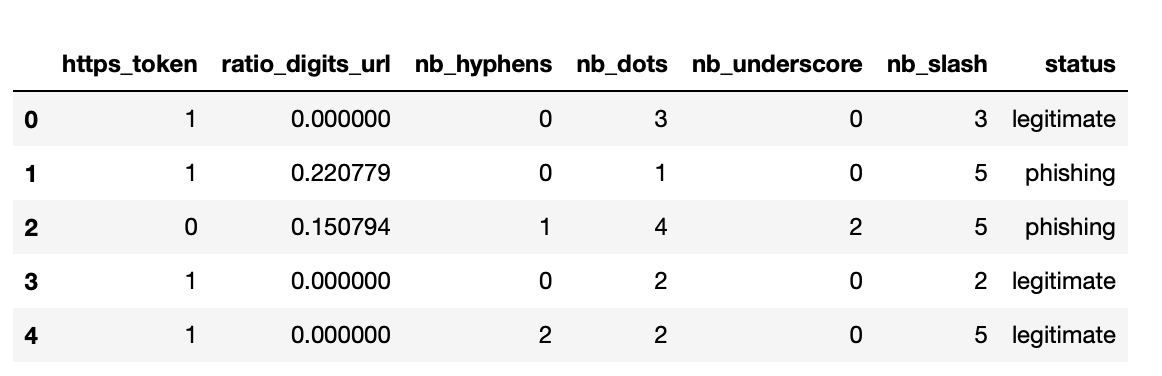
\includegraphics{dataset.png}

\subsection{Machine Learning Algorithms}
One machine learning we will be using is KNN-classifier. 

\subsection{Implementation Details}
The data is split into a training size of 75 percent, and a dataset for testing of size 25 percent of the entire dataset. To optimize this algorithm, The "best k" value is 18, which is how many neighbors are used in the sklearn.neighbors.KNeighborsClassifier python function. We are collecting the best value of k "best_k", by computing the cross_val_score accuracy for k in range (1,61) which is shown in the graph below:
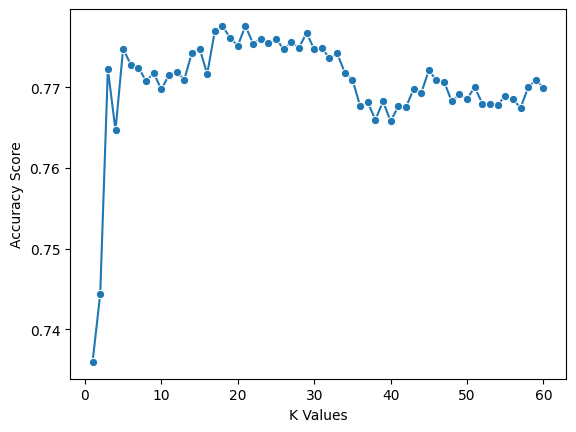
\includegraphics{best-k-value.png}

Training this model yielded Accuracy: 0.7925122463261022, Precision: 0.8117998506348021, and Recall: 0.761204481792717.

\section{Comparison}  
This section includes the following: 1) comparing the performance of different machine learning algorithms that you used, and 2) comparing the performance of your algorithms with existing solutions if any. Please provide insights to reason about why this algorithm is better/worse than another one.

\section{Future Directions}
This section lays out some potential directions for further improving the performance. You can image what you may do if you were given extra 3-6 months.

\section{Conclusion}
This section summarizes this project, i.e., by the extensive experiments and analysis, do you think the problem is solved well? which algorithm(s) might be better suitable for this problem? Which technique(s) may help further improve the performance? \\

Last but not the least, don't forget to include references to any work you mentioned in the report.
  

\bibliographystyle{IEEEtran}
\bibliography{}


\end{document}


